% mainfile: ../../../../master.tex
\subsection{RNA quantification Nanodrop}
% The part of the label after the colon must match the file name. Otherwise,
% conditional compilation based on task labels does NOT work.
\label{task:20180113_cj1}
\tags{lab,qnt,rna}
\authors{cj}
%\files{}
%\persons{}

\begin{figure}[H] % position of the figure 
    \centering
    \caption{Screenshots of the NanoDrop analysis of RNA samples extracted from bacterial cultures}
    \label{fig:CJ20180113_RNA}
    \begin{subfigure}[b]{0.3\textwidth}
        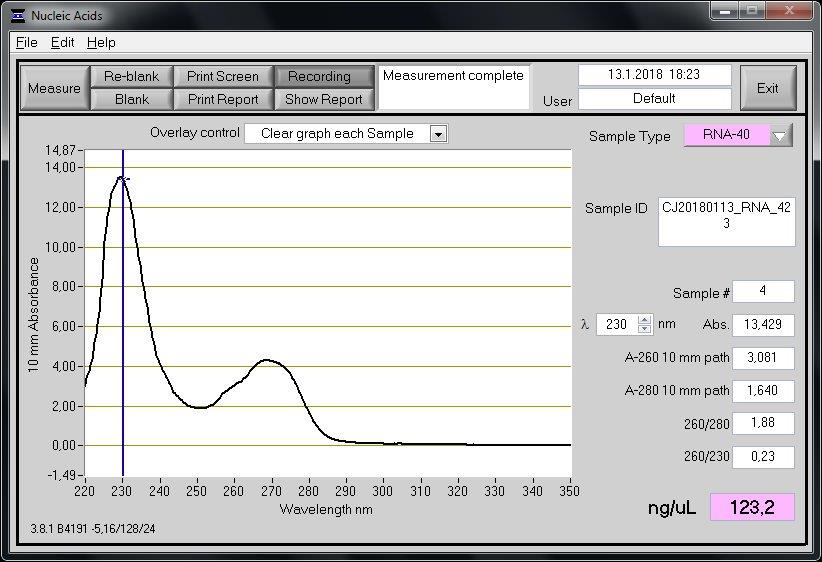
\includegraphics[width=\textwidth]{graphics/screenshots/CJ20180113_RNA_423.jpg}
        \caption{CJ20180113\_RNA\_423}
        \label{sfig:CJ20180113_RNA_423}
    \end{subfigure}
    ~ 
    \begin{subfigure}[b]{0.3\textwidth}
        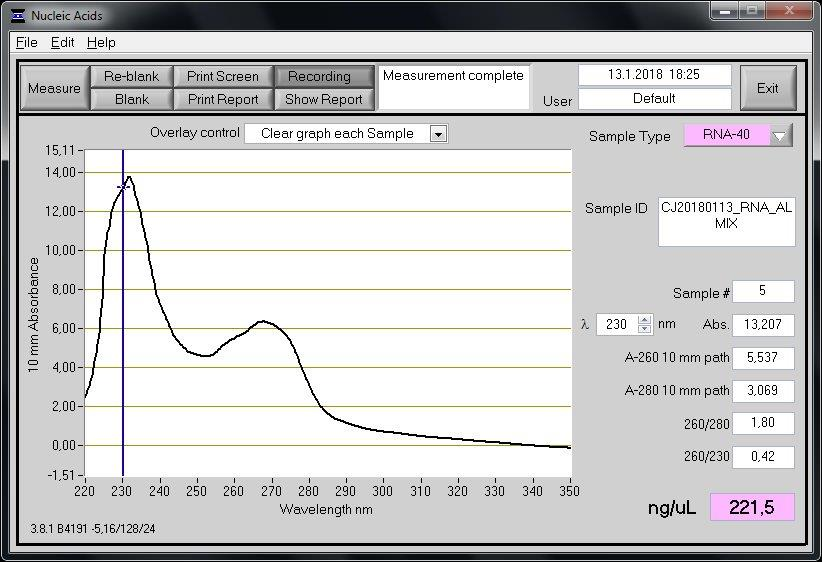
\includegraphics[width=\textwidth]{graphics/screenshots/CJ20180113_RNA_ALMIX.jpg}
        \caption{CJ20180113\_RNA\_ALMIX}
        \label{sfig:CJ20180113_RNA_ALMIX}
    \end{subfigure}
     ~ 
    \begin{subfigure}[b]{0.3\textwidth}
        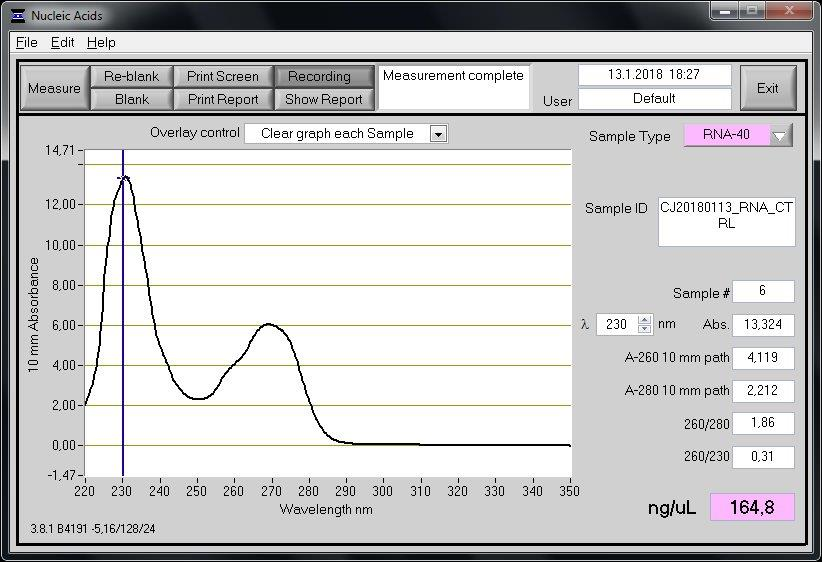
\includegraphics[width=\textwidth]{graphics/screenshots/CJ20180113_RNA_CTRL.jpg}
        \caption{CJ20180113\_RNA\_CTRL}
        \label{sfig:CJ20180113_RNA_CTRL}
    \end{subfigure}
\end{figure}

\begin{table}
\caption{res/nanodrop/CJ20180113.txt}
\label{tab:}
\centering
\begin{tabular}{l l l l l l l l l l l l l }
\toprule
Sample ID & Time  & ng/ul  & A260  & A280  & 260/280  & 260/230  \\ \midrule
\texttt{CJ20180113\_BLANK} & 18:21 & -0,06 & -0,001 & -0,006 & 0,22 & 0,22 \\
\texttt{CJ20180113\_RNA\_423} & 18:22 & 123,24 & 3,081 & 1,640 & 1,88 & 0,23 \\
\texttt{CJ20180113\_RNA\_ALMIX} & 18:25 & 221,46 & 5,537 & 3,069 & 1,80 & 0,42 \\
\texttt{CJ20180113\_RNA\_CTRL} & 18:26 & 164,76 & 4,119 & 2,212 & 1,86 & 0,31 \\
\texttt{} &  &  &  &  &  &  \\

\bottomrule
\end{tabular}
\\
User: Default - Date: 13.1.2018 - Constant:  - Cursor position: 230 \
\end{table}